\chapter{ Конструкторский раздел}
\label{cha:design}

Исходя из существующих методов, описанных в аналитическом разделе, можно сделать вывод о том, что оптимальное решение проблемы колоризации графических новелл будет содержать в себе комбинацию двух методов. Метод колоризации с использованием цветовых подсказок можно оптимизировать, используя вместо цветовых подсказок гистограмму распределения цветов, полученную на основе графа опорного изображения (граф получить, исходя из метода с использованием опорного изображения, графика и квадратичного программирования). Тоесть время работы модифицированного метода должно сократиться ввиду исключения или сведения к минимуму гонки генератора и дискриминатора. Гонка возникает на этапе работы с цветовыми подсказками. 




Представим задачу разработки автоматизированного метода колоризации  графических новелл на Рисунок 2.1 в качестве "IDF0" диаграммы.
\newpage
\begin{figure}[ht!]
	\centering{ 
		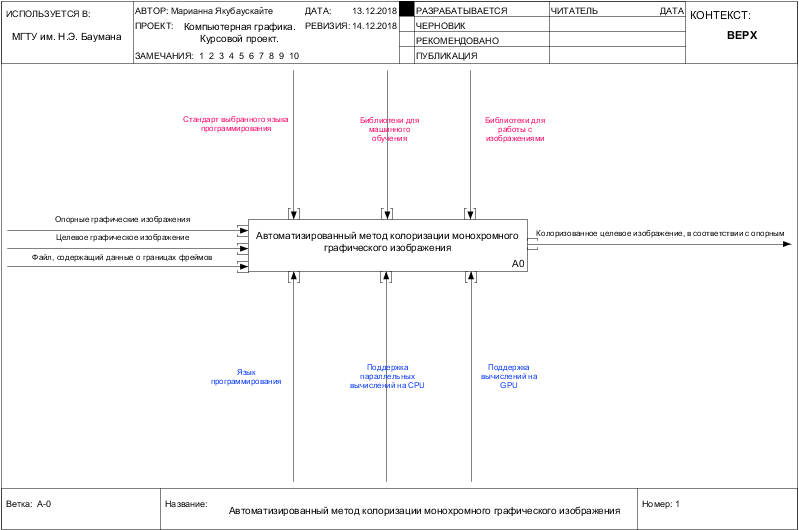
\includegraphics[width=0.7\textwidth]{img/01_A-0.png}
		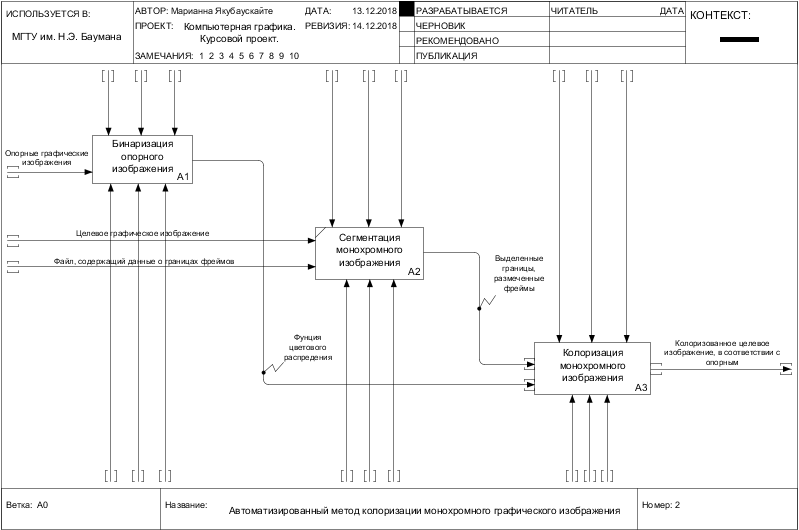
\includegraphics[width=0.7\textwidth]{img/02_A0.png}
		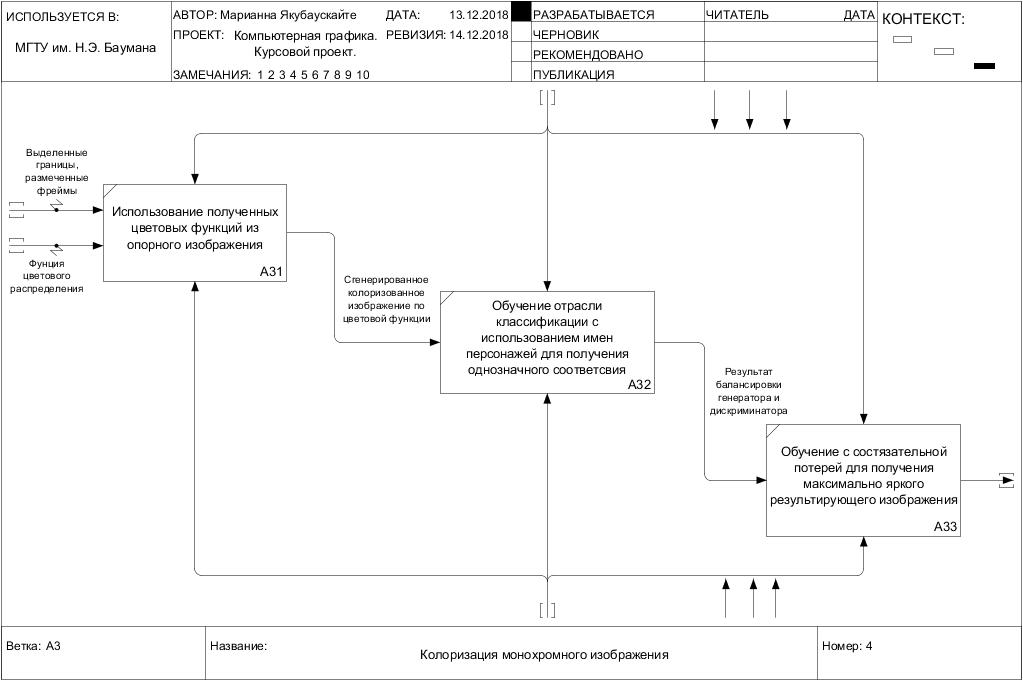
\includegraphics[width=0.7\textwidth]{img/04_A3.jpg}
		\caption{IDF0 диаграмма метода.}}
\end{figure}

\newpage
 \section{Описание общего алгоритма работы.}
 Общая модель работы представлена на Рисунок 2.2.
 
 На вход требуется подать монохромное изображение манги и опорные цветные изображения, причем количество опорных изображений должно удоволетворять условию-соответсвию: один фрейм = одно опорное изображение. Далее проводится сегментация изображения по фреймам (координаты самих фреймов могут быть предствлены на языке разметки, к примеру быть описаны в $*.json$ файле). Каждому фрейму проводится соотвествие с его опорным изображением, из опорного изображения методом бинаризации извлекается цветовая гистограмма - называемая в частности, цветовой функцией и представляющая собой цветовую палитру, использованную для раскраски опорного изображения.Затем происходит колоризация монохромного сегмента в соответсвии с цветовой гистограммой, наносятся поверх контуры и текст. 

\begin{figure}[ht!]
	\centering{ 
		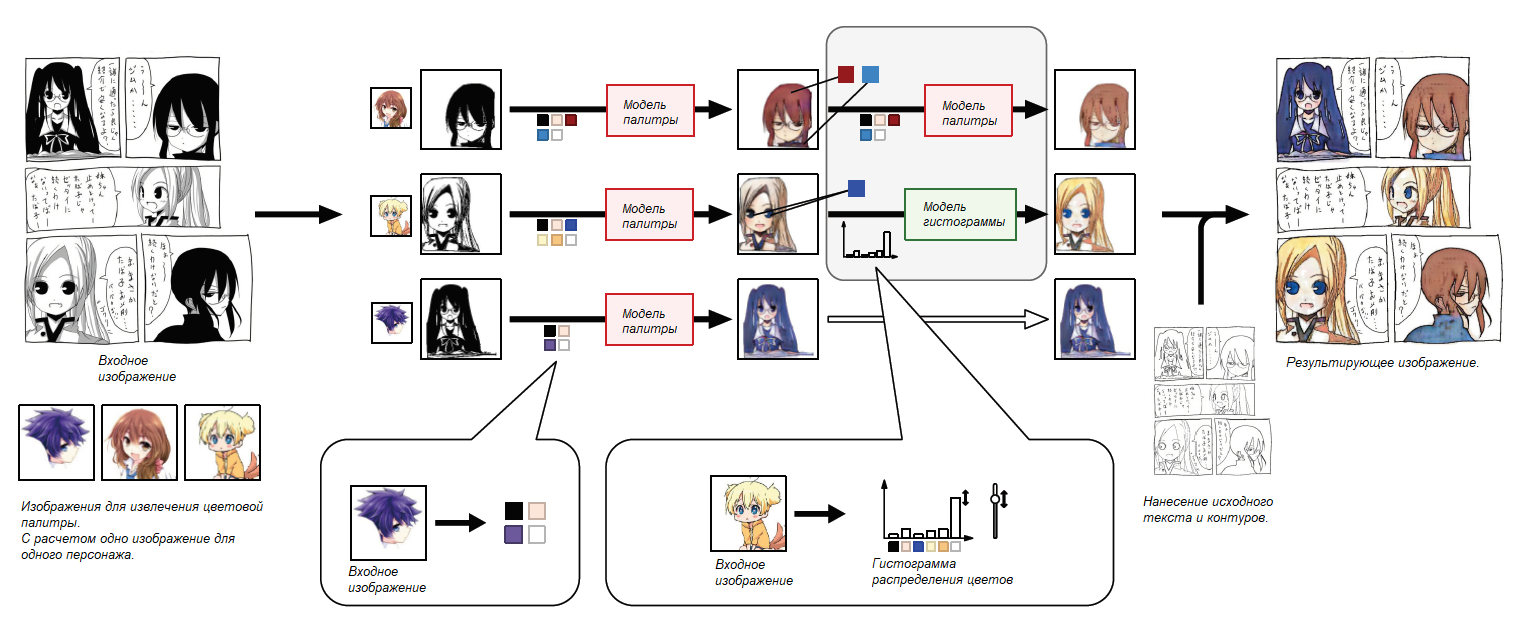
\includegraphics[width=1\textwidth]{img/7.png}
		\caption{Общая модель работы.}}
\end{figure}

Архитектура модели нейронной сети позаимствована у метода колоризации с использованием цветовых подсказок - их модель поддерживает концепцию четырех сетей, представляющей слои одной единой сверточной нейронной сети:
\begin{enumerate}
	\item глобальная сеть функций;
	\item низкоуровневая сеть функций;
	\item сеть среднего уровня;
	\item cеть раскраски.
\end{enumerate}

Основываясь на методе, описанном в вышеупомятой работе, и используя метод переноса цветовой функции с опорного изображения на монохромное, в архитектуру будут добавлены следующие элементы:
\begin{enumerate}
	\item использование цветовой палитры от опорных изображений;
	\item обучение классификации с использованием имен персонажей (использование data-set $"manga$ $109"$);
	\item обучение с учетом состязательной потери для получения визуально более ярких и насыщенных цветов.
\end{enumerate}

Архитектура модифицированной нейронной сети представлена на Рисунке 2.3.

\begin{figure}[ht!]
	\centering{ 
		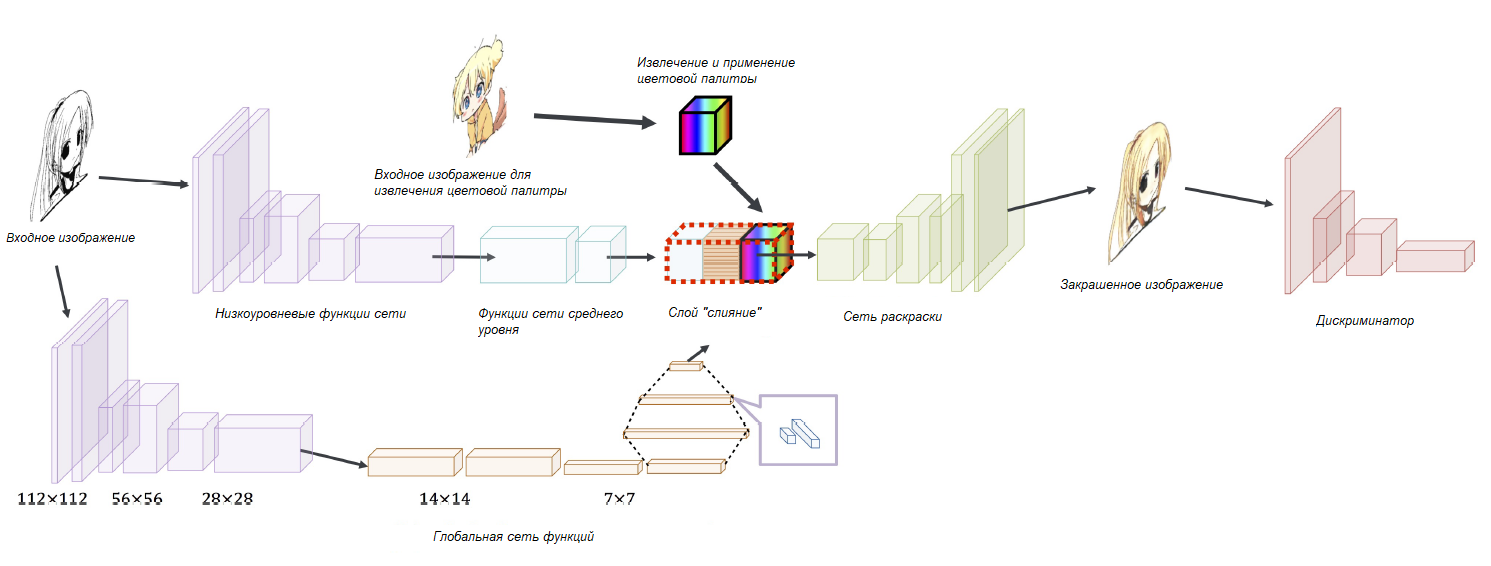
\includegraphics[width=1\textwidth]{img/8.png}
		\caption{Архитектура нейронной сети}}
\end{figure}
